Nachdem die theoretischen Grundlagen und der Aufbau des ALICE Experiment n\"aher erl\"autert wurden, wird im folgenden die Vorgehensweise erkl\"art, wie $\pi^{0}$ gemessen werden.
\newline
Die in Abschnitt \ref{s3s1s2} genannten Auswahlkriterien von \textit{Clustern}, filtern die \textit{Cluster} so, dass haupts\"achlich \textit{Cluster} die aus einen Photon, Elektron oder Positron bestehen, \"ubrig bleiben.
\newline
\begin{figure}[thp] \label{figInvMassPt}
\centering
\begin{subfigure}{.5\textwidth}
	\centering
	\includegraphics[width=.95\linewidth]{hInvMass_pT_Signal.pdf}
	\caption{}
	\label{figInvMassPt_a}
\end{subfigure}%
	\begin{subfigure}{.5\textwidth}
	\centering
	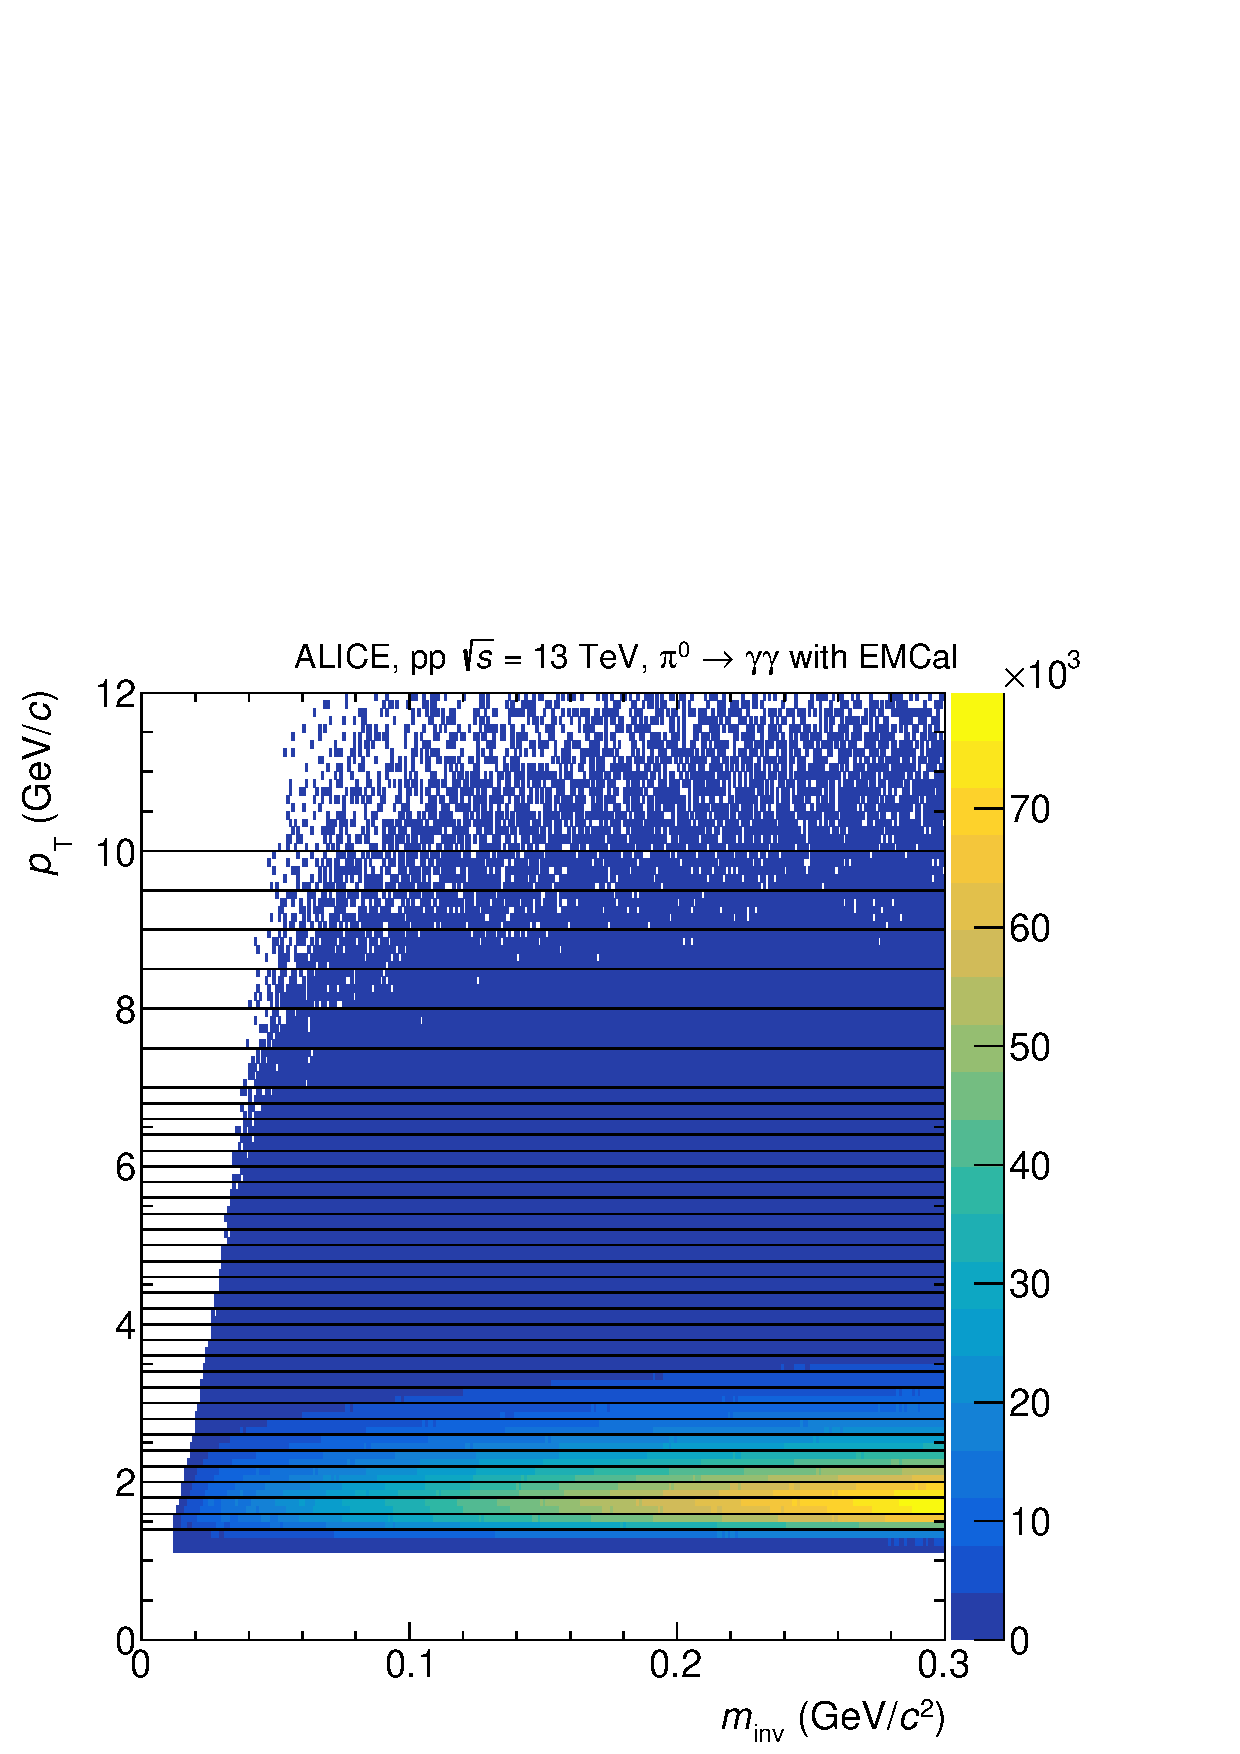
\includegraphics[width=.95\linewidth]{hInvMass_pT_Bkg.pdf}
	\caption{}
	\label{figInvMassPt_b}
\end{subfigure}
\caption{\newline{\bf (a)}: $p_\text{T}$ und $m_\text{inv}$ als Funktion von der Anzahl von rekombinierten  Cluster-Paaren aus der gleichen Kollision.
Die schwarze Linie liegt bei $m_{\text{inv}}=0,135\text{ GeV/}c^{2}$, was der $\pi^{0}$ Masse entspricht, wo eine deutliche Peakstruktur zu Erkennen ist.
\newline
{\bf (b)}: $p_\text{T}$ und $m_\text{inv}$ als Funktion von der Anzahl von rekombinierten  Cluster-Paaren aus unterschiedlichen Kollision.}
\end{figure}
Um $\pi^{0}$ messen zu k\"onnen, werden aus den Photonenkandidaten, die zu den genannten \textit{Clustern} korrespondieren, die invariante Masse und der Transversalimpuls nach Gleichungen \ref{eq_invmass} und \ref{eq_pt} bestimmt.
Da die Information, ob und welche Photonenkandidaten von einem $\pi^{0}$ stammen, fehlt, werden alle Photonenkandidaten eines \textit{Events} mit einander kombiniert.
Dieses Vorgehen wird als \textit{same event method} bezeichnet.
Abbildung \ref{figInvMassPt_a} zeigt die Anzahl solcher Rekombinationen in abh\"angigkeit der invarianten Masse $m_{\rm{inv}}$ und des Transversalimpulses $p_{\rm{T}}$.
Durch die Kombination aller Photonenkandidaten eines \textit{Events} gibt es sowohl Rekombinationen zusammengeh\"origer Photonenkandidaten, als auch unabh\"angiger Photonenkandidaten.
Es zeichnet sich eine Anh\"aufung der Datenpunkte um $m_{\rm{inv}}\approx 0,135\rm{GeV}/c^{2}$, also um die Masse von $\pi^{0}$, ab.
Dieser Anh\"aufung liegen vor allem Rekombinationen zusammengeh\"origer Photonenkandidaten zugrunde.
\newline
Um die Anzahl produzierter $\pi^{0}$ bestimmen zu k\"onnen, muss die Anzahl der Kombinationen unabh\"angiger Photonenkandidaten abgezogen werden.
Die Anzahl der Kombinationen unabh\"angiger Photonenkandidaten wird als kombinatorischer Untergrund oder auch unkorrelierter Untergrund bezeichnet.
Dazu wird die Anzahl der Kombinationen unabh\"angiger Photonenkandidaten abgesch\"azt mit der sogenannten \textit{mixed event method}.
In dieser Methode werden Photonenkandidaten aus unterschiedlichen \textit{Events} miteinander kombiniert, sodass keine Korrelation zwischen den Photonenkandidaten besteht.
Abbildung \ref{figInvMassPt_b} zeigt eine solche Verteilung, bei der Photonenkandidaten aus unterschiedlichen Kollisionen miteinander kombiniert wurden.
Da mehr Kombinationsm\"oglichkeiten in der \textit{mixed event method} zur Verf\"ugung stehen, gibt es mehr Eintr\"age in der zweiten Verteilung.
\begin{figure}[tbp]
\centering
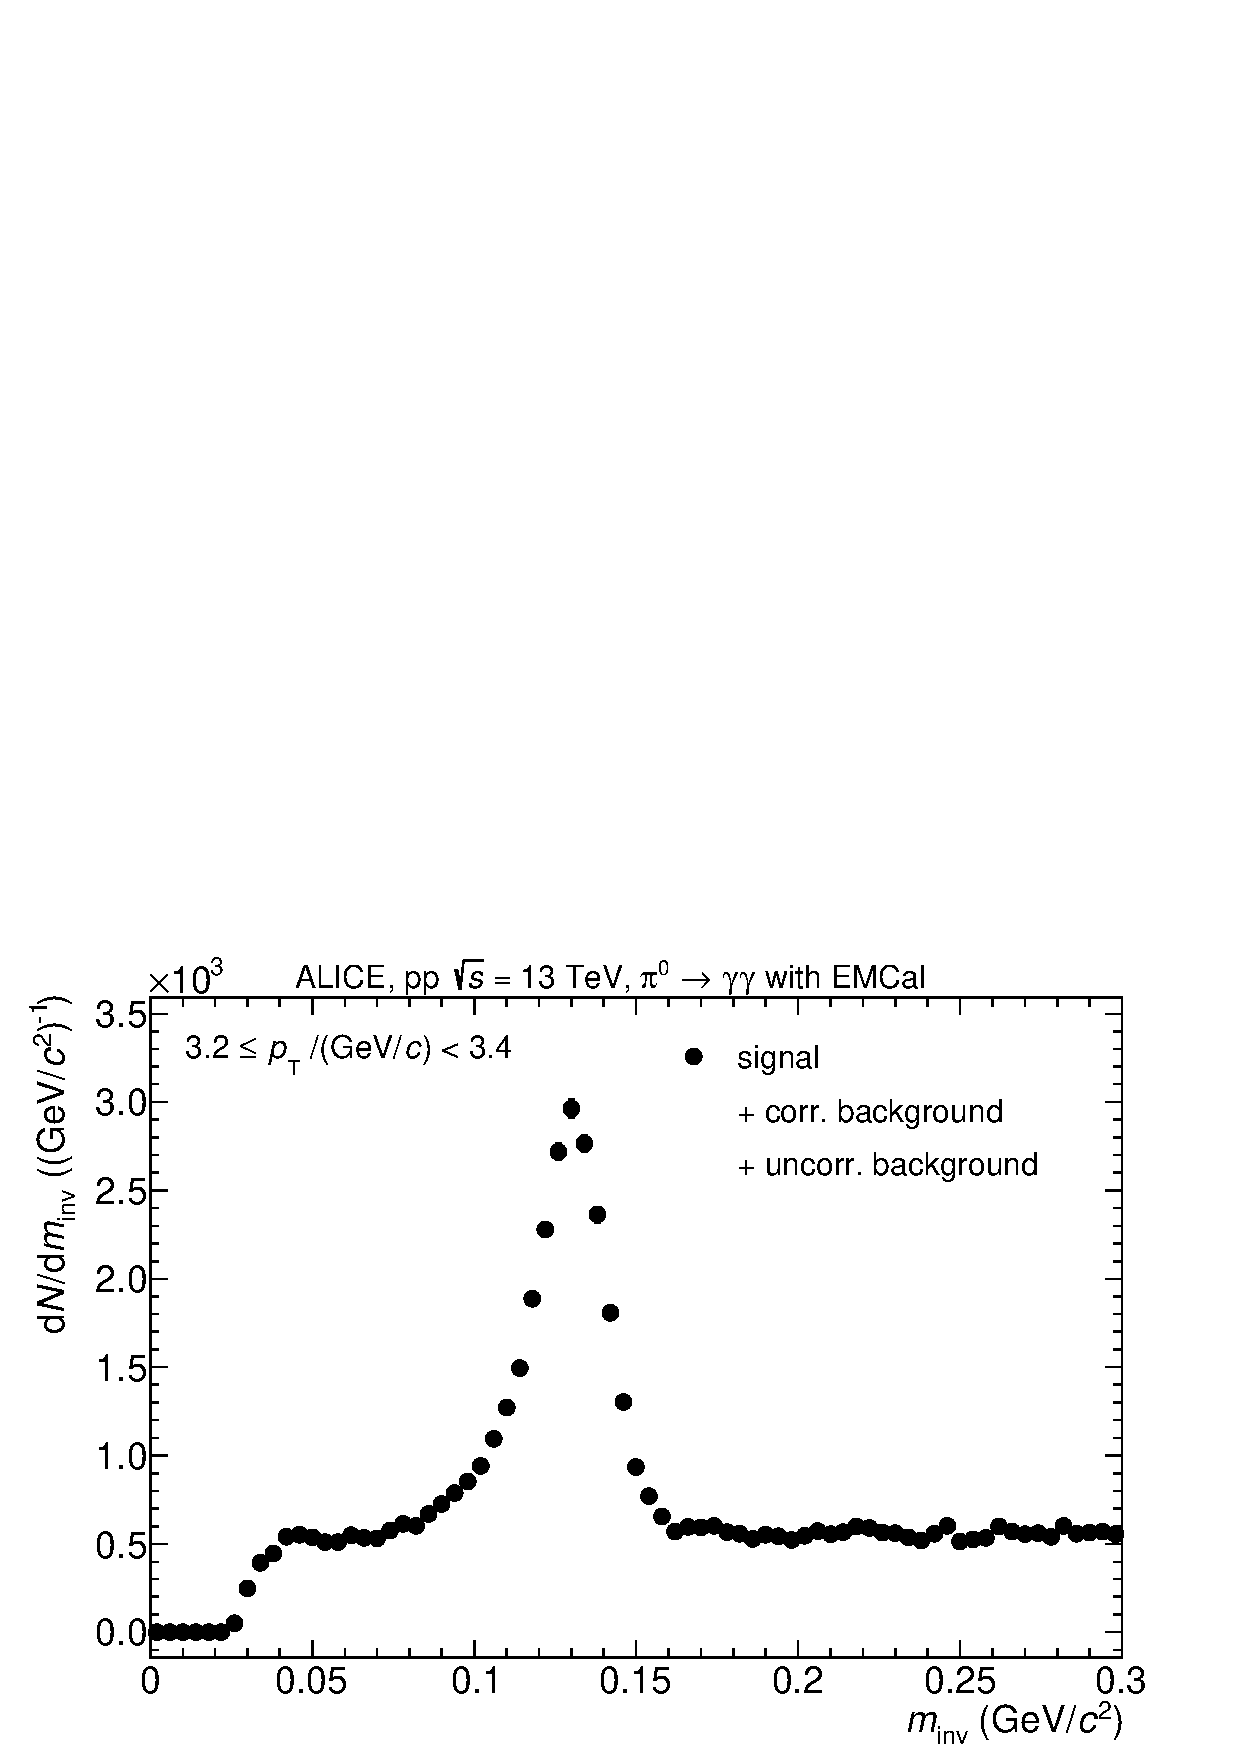
\includegraphics[width=.6\linewidth]{hSignalPlusBkg.pdf}
\caption{Projektion von Abbildung \ref{figInvMassPt_a} im $p_{\text{T}}$-Intervall (3.2 - 3.4) $(\text{GeV/}c)$. Es ist ein deutlicher Peak um $m_{\pi^{0}} \approx 0,135\text{GeV/}c^{2}$ zu erkennen, aber auch Untergrund, da das Signal zu h{\"o}heren Massen gau{\ss}f{\"o}rmig abklingen sollte. Bei $m_{\text{inv}} < m_{\pi^{0}}$ kann Signal vorliegen, das aus konvertierten Photonen besteht, weshalb eine Aussage {\"u}ber die Form, bzw. den Untergrund dort schwer m{\"o}glich ist.}
\label{figSignalPlusBkg}
\end{figure}
\newline
Um den unkorrelierten Untergrund abzusch\"atzen wird in einzelnen $p_{\rm{T}}$-Intervallen 
Um $\pi^{0}$s in einzelnen $p_{T}$-Intervallen z{\"a}hlen zu k{\"o}nnen wird die Verteilung in entsprechende Abst{\"a}nden auf die Y-Achse projiziert.
Die Intervalle werden so gew{\"a}hlt, dass sie m{\"o}glichst klein sind, w{\"a}hrend die statistischen Unsicherheiten nicht zu gro{\ss} werden.
Abbildung \ref{figSignalPlusBkg} zeigt eine Verteilungen der invarianten Masse, die aus Signal, sowie sogenanntem korrelierten und unkorrelierten Untergrund besteht.
Trotz der Untergr\"unde ist ein deutlicher Peak im Bereich der Pionenmasse von ca. $135\rm{MeV}/c^{2}$ zu erkennen.
Die Bestimmung der beiden Untergr\"unde, vor allem des korrelierten Untergrunds, ist eine wichtige Aufgabe in der Analyse von neutralen Pionen.
Das Parametrisieren einer Funktion hat sich als g\"angie Methode zur Bestimmung des korrelierten Untegr\"unds entwickelt und wird im folgenden als Standardmethode bezeichnet.
In dieser Arbeit wird der korrelierte Untergr\"und sowie das reine $\pi^{0}$-Signal mit Hilfe von sogenannten \textit{Monte Carlo Templates} bestimmt.
Die Ergebnisse der Analyse mit Hilfe von Monte Carlo Templates, sowie mit der Standardmethode werden miteinander vergleichen, um eine Aussage \"uber den m\"oglichen Nutzen von Analysen mit Hilfe von Monte Carlo Templates treffen zu k\"onnen.
Im folgenden Abschnitt wird sowohl die Standardmethode kurz, als auch die Methode mit Hilfe von Monte Carlo Templates n\"aher erl\"autert.
